\documentclass{proyectotesis}
%\usepackage[backend=biber,sortlocale=en,natbib=true,citestyle=numeric-comp,languaje=english,,sorting=none]{biblatex}
%\addbibresource{refs.bib}

%%%%%%%%%%%%%%%%%%%%%%%%%%%%%%%%%%%%%%%%%%%
%%%%%%%%%%%%%%%%%%%%%%%%%%%%%%%%%%%%%%%%%%%
%%%%%%%%%%%%%%%%%%%%%%%%%%%%%%%%%%%%%%%%%%%

\title{Análisís de polarización en la Cámara de Diputados de Chile}
\author{Benjamín Matías Ortiz Edwards}
\pronom{el}
\postgrado[Magíster]{en Ciencias con mención en Física.}
%\directora{}
%\director{}
\directores{Dra. Denisse Pastén y Dr. Víctor Muñoz}
%\codirector{}
\duracion{Primer y segundo semestre 2022.}
\lugar{Grupo Planets (www.planets.cl), Departamento de Física, Facultad de Ciencias, Universidad de Chile.}
\direccion{Las Palmeras 3425, Ñuñoa, Santiago, Chile. \\Dirección Postal: Casilla 653, Santiago, Chile. Fono: (56-2) 2978 7276.}

%%%%%%%%%%%%%%%%%%%%%%%%%%%%%%%%%%%%%%%%%%%
%%%%%%%%%%%%%%%%%%%%%%%%%%%%%%%%%%%%%%%%%%%
%%%%%%%%%%%%%%%%%%%%%%%%%%%%%%%%%%%%%%%%%%%

\nacimiento{10 de febrero, 1997}
\RUN{19.359.906-0}
\telefono{(+56\;9)\:8656\;0757}
\email{bedw@bedw.me}

\begin{document}

\maketitlepage
\makepersonalinfo

%%%%%%%%%%%%%%%%%%%%%%%%%%%%%%%%%%%%%%%%%%%
%%%%%%%%%%%%%%%%%%%%%%%%%%%%%%%%%%%%%%%%%%%
\subsection{Educación}
\begin{cvlist}{}
\item[\textbf{Educación Superiror}] 
\item[\textbf{2015 - 2020}] Licenciatura en Ciencias con mención en Física, Universidad de Chile.
\item[\bf Educación Escolar]
\item[\textbf{2010 - 2014}]  Enseñanza Básica y Media, Colegio Compañia de María Seminario.
\end{cvlist}

\subsection{Experiencia Profesional}
\begin{cvlist}{}
\item[\textbf{2020}]   \textbf{Ayudante},  Métodos de la Física Matemática II, Departamento de Física, Facultad de Ciencias, Universidad de Chile, Segundo Semestre.
\item[\textbf{2021}]   \textbf{Ayudante},  Métodos de la Física Matemática II, Departamento de Física, Facultad de Ciencias, Universidad de Chile, Segundo Semestre.
\item[\textbf{2019}]  \textbf{Practicante}, "Practicas de Verano", DFC-DFI, Universidad de Chile.   
\item[\textbf{2021 - Presente}] \textbf{Programador analísta}, Centro de Inteligencia Territorial, Universidad Adolfo Ibañez. 

\end{cvlist}

\subsection{Presentaciones a Congresos}

\begin{cvlist}{}
\item[\textbf{2020}] \textbf{Ortiz Edwards, B.}, Pastén, D., y Muñoz, P. S. A complex network approach on the analysis of the Chilean presidential elections, using Twitter Data, {\it Complex Networks 2019}, Lisboa, Portugal, 10-12 de diciembre.

\end{cvlist}

\newpage

\section{Exposición General del Proyecto}
\subsection{Resumen}

\subsection{Introducción}
%La teoría de grafos busca abstraer esquemáticamente conjuntos de datos mediante criterios geométricos específicos a partir de nodos o vértices y algún tipo de relación que pueda presentar con otros nodos mediante aristas, donde estas mismas pueden presentar una orientación definida, existiendo un nodo fuente y un nodo de destino. El inicio de esta teoría fue en el año 1736 en manos de Leonhard Euler, en un artículo que trató el problema conocido como los puentes de Königsberg \cite{euler1741solutio} cuyo propósito inicial fue determinar la ruta más eficiente para cruzar todos los puentes de la ciudad, con la restricción de cruzarlos una sola vez. Euler demostró la imposibilidad del caso, sin embargo este hito ha permitido el desarrollo de importantes estudios, permitiendo desde entonces grandes avances en diversas áreas, tales como urbanismo \cite{bro2021surname},  economía \cite{gomez2020reducing}, redes biológicas \cite{ilias2020adaptive} e incluso en la selección de enfoques fundamentales en  la salud, como la propagación de enfermedades \cite{liu2020new}, entregando soluciones sustanciales a problemas complejos.\\


%Existen diferentes tipos de grafos y estructuras de representación con los que trabajar, dependiendo de las características que se buscan explorar en cada investigación. En el análisis de los datos relevantes para este trabajo, lo que interesa es modelar series de tiempo como redes complejas. Para ello, se cuenta con las herramientas de la familia de algoritmos de visibilidad, que convierten series de tiempo en grafos donde la estructura de la serie se conserva en la topología del grafo \cite{lacasa2008time}, logrando construir un puente natural entre la teoría de redes complejas y el análisis de series de tiempo. %En este grafo cada nodo corresponde, en el mismo orden, a datos en serie, y se conectan dos nodos si existe visibilidad (oblicua) entre los datos correspondientes, es decir, si existe una línea recta que conecta los datos en serie, siempre que que esta ``línea de visibilidad" no cruce ninguna altura de datos intermedia.\\ %\cite{lacasa2012time}

Las redes complejas son muy útiles para caracterizar sistemas con muchos elementos que interactuan entre si. Estas nos permiten modelar distintos sistemas mediante una representación de grafos, con nodos y conexiones, para luego obtener distintas propiedades del sistema a partir de métricas, o propiedades estadísticas o topológicas de la red.\\

Este proyecto busca estudiar la polarización de la Cámara de Diputados de Chile, a partir de las interacciones entre los miembros de esta, haciendo uso de redes. 
Como contexto, la mayoria trabajos que estudian parlamentos de distitos paises usando analisis de redes (legislative networks~\cite{Neal_2020, Waugh_2009, Aleman_2013, Zhang_2008, Fowler_2006, Andris_2015, Briatte_2016, LeFoulon_2019}
), tienen más o menos en común la forma en que crean las redes legislativas. En estas los \textbf{parlamentarios se representan como nodos, y las relaciones entre ellos como conexiones}. El criterio a partir del cual se definen las relaciones entre los parlamentarios varía de trabajo en trabajo, pero los más usados consisten en definirlas a partir del patrocinio en conjunto a las propuestas de ley~\cite{Neal_2020, Zhang_2008, LeFoulon_2019,Fowler_2006}, o partir de la coordinacion (o descordinación) de los parlamentarios al momento de votar~\cite{Waugh_2009, Andris_2015}. En este proyecto proponemos usar el segúndo criterio.\\

Para estudiar la polarización de una red es necesario \textbf{detectar comunidades} en ella, a partir de las conexiones y sus pesos (intensidades). Luego, una red se considera polarizada cuando los nodos de una misma comunidad tienen interacciones más fuertes entre sí, mientras que más debiles (o nulas) con los nodos de distintas comunidades. Esta concepción de polarización es llamada ``polarización debil'' por Neal~\cite{Neal_2020}. Sin embargo, en su trabajo tambien propone un segundo tipo de polarización, lo que denomina ``polarización fuerte''. Esta consiste en que, además de haber muchas conexiones (e intensas) entre los nodos de una misma comunidad, entre nodos de comunidades diferentes existan conexiones pero de peso negativo.\\

Ante esto nos preguntamos: ¿Es posible medir la polarización politica de la Camara de de Diputados de Chile, usando redes complejas?. Y de ser posible, ¿Esta polarización de tipo debil o fuerte?.\\

Para detectar comunidades hay diversos algoritmos, pero sin duda los mas utilizados son aquellos que maximizan la Modularidad ($Q$)~\cite{Newman_2004, Clauset_2004, Duch_2005, Blondel_2008, Arab_2012, Chen_2014}. Esta cantidad fue definida inicialmente por Newman y Girvan~\cite{NewmanGirvan2004} y da cuenta de que tan ``modular'' es una red según una partición de comunidades. En este contexto, diremos que $\sigma_i$ es una etiqueta indicando que comunidad le fue asignada al nodo $i$, y luego la partición de comunidades será el conjunto $\sigma = \{\sigma_i\}$ indicando las comunidades asignadas a todos los nodos de la red.

Como se mencionó anteriormente, muchos algoritmos utilizan esta medida para detectar comunidades. En terminos sencillos, estos prueban distintas comunidades y evaluan la modularidad. Luego, la partición de comunidades (el conjunto $\sigma = \{\sigma_i\}$) que maximiza la modularidad es el output del algoritmo.


Por otro lado, Reichardt y Bornholdt desarrollaron un algoritmo que tiene sus bases en mecánica estadistica. Este consiste en la definición de un hamiltoniano que debe minimizarse para obtener la partición de comunidades óptima. Además, los autores demuestran que la minimización de la energía (del hamiltoniano) es equivalente a la maximización de la Modularidad.\\

Ahora, con las comunidades ya identificadas, ¿Como medimos la polarización?. Varios autores usan la misma medida de Modularidad como un indicador de polarización, considerando que mientras más alta sea la Modularidad, la red está más polarizada. Sin embargo, esto solo servirá para medir polarización debil, ya que la Modularidad como tal no está definida para conexiones con pesos negativos. Ante esto, Neal propone usar el Índice del triángulo para cuantificar la polarización fuerte. 

Ante esto nos preguntamos: ¿Habrá un método basado en mecánica estadística, de forma similar al planteado por Reichardt, que sea equivalente a la maximización del índice del triángulo?. Por último, también, ¿Es el índice del triángulo la forma más optima de cuantificar la polarización fuerte?

\subsection{Objetivos}

En el contexto del estudio de interacciones entre los miembros de la Cámara de Diputados de Chile, se busca evaluar los algoritmos de detección de comunidades basados en la maximización de modularidad como una medida ``óptima'' de polarización política. Para ello se propone comparar los valores de modularidad y , con el índice del triángulo, al considerar interacciones negativas (repulsivas). 
También se busca desarrollar una medida de polarización basáda en mecánica estadistica, basandonos en trabajos similares.

\subsubsection*{Objetivos Específicos}
\begin{itemize}
\item    {\bf Análisis de Redes Complejas.} Caracterizar la interacción entre miembros de la Cámara de Diputados de Chile, por medio de la representación del sistema como red compleja, a partir de los datos públicos de las votaciones en sala, u otros similares.

\item{\bf Comparación entre la modularidad y el índice del triángulo.} Con la red construida se propone utilizar métodos de tección de comunidades, para luego medir la modularidad, y comparar esta cantidad con el índice del triángulo. El proposito de esto es identificar nociones de polarización debil o fuerte con las herramientas que en este momento tenemos a disposición.

\item {\bf Desarrollo de nuevo algoritmo de detcción de comunidades, basada en Mecánica Estadística.} De forma similar a lo relizado po Reichardt, se busca crear un hamiltoniano que incorpore conexiones negativas, pero que se relacione con la maximización del índice del triangulo o con la maximización otra medida que de cuenta de la polarización fuerte.

\end{itemize}

\subsection{Metodología}
\subsubsection{Análisis de Redes Complejas.}
Se busca caracterizar la interacción entre miembros de la Cámara de Diputados de Chile, por medio de la representación del sistema como red compleja, a partir de los datos públicos de las votaciones en sala. En terminos simple, consideraremos los parlamentarios los nodos de la red, y entos tendrán conexiones según la coordinacón (o descoordinación) al momento de votar en Sala.

Los votos de una votación en Sala $k$ los representaremos mediante el vector 
\begin{equation}
    v^k = \{u_1,\dots,u_n\}
\end{equation}
con $u_i$ la opción que el o la parlamentaria $i$ votó. Esta será 1 si el voto fue a favor, -1 si fue en contra y 0 en caso de abstención o ausencia.

Realizando el producto externo de $v^k$ consigo mismo, se obtiene la matriz $M^k$ que representa la coordinación de los parlamentarios en la votación $k$. De esta forma la coordenada $M^k_{ij}$ será 1 si los parlamentarios $i$ y $j$ votaron lo mismo, -1 si votaron opciones opuestas, y 0 si alguno se abstuvo o estuvo ausente. Entoces, ahora, para $m$ votaciones, tendremos la siguiente matriz.
\begin{equation}
    A_{ij} = \sum_k^m M^k_{ij} \label{adj}
\end{equation}
Con esta matriz ya podemos crear la red. Si una coordenada $A_{ij}\neq 0$ entonces creamos una conexión entre los nodos $i$ y $j$ , y con una peso igual a $A_{ij}$. Para los casos $A_{ij} = 0$, simplemente no se crea ninguna conexión entre los nodos $i$ y $j$.\\

La Modularidad se define por
\begin{equation}
    Q = \frac{1}{2m}\sum_{ij} \left( A_{ij} - \frac{k_i k_j}{2m}  \right) \delta(\sigma_i,\sigma_j) \label{mod}
,\end{equation}
con $k_i$ la suma de los pesos de las conexiones del nodo $i$, $m = \frac{1}{2} \sum_i k_i$. También tenemos $\sigma_i$ que indíca a que comunidad pertenece el nodo $i$, y $\delta(\sigma_i,\sigma_j)$ se define de tal forma que es 1 si los nodos $i$ y $j$ pertenecen a la misma comunidad, o 0 en caso contrario.

Queda pendiente definir cuantas y cuales votaciones se considerarán para armar la red. Se plantea también la idea de armar varias redes a partir de votaciones ocurridas en periodos o intervalos temporales distintos. Al agregar la dimensión temporal podemos relacionar los posteriores analisis relacionados a la polarización, con la temporalidad de las votaciones y su cercacanía con hitos políticos relevantes.

\subsubsection{Comparación entre la modularidad y el índice del triángulo} 
Luego de crear la red a partir de la matriz de adjacencia de la ecuación \eqref{adj}, se busca medir la modularidad y el índice del triángulo para compararlos. Para ello se propone momentaneamente ``ignorar'' las conexiones negativas, remplazando todas las entradas de $A_{kl} < 0$.\\ 

Ahora, con esta red de solo conexiones de peso positivo, detectamos comunidades con el método ``spin-glass'', y con la partición de comunidades resultante, calculamos la modularidad. 

Luego, ahora si considerando las conexiones de peso negativo, se pretende medir el índice del triángulo con la particion de comunidades obtenida anteriormente.

\subsubsection{Desarrollo de nuevo algoritmo de detcción de comunidades, basada en Mecánica Estadística} 
Reichardt y Bornholdt desarrollaron un Hamiltoniano que al minimizarlo nos permite obtener la partición de comunidades óptima de una red, a partir de las conexiones entre los nodos. También demostraron que minimizar su Hamiltoniano es equivalente a maximizar la modularidad bajo ciertas condiciones. 
Al momento de desarrollar el Hamiltoniano, los autores lo abordaron de la siguiente manera
\begin{align}
\begin{split}
    \mathcal{H}(\{\sigma\}) = &- \sum_{i\neq j} a_{ij}\underbrace{A_{ij}\delta(\sigma_i,\sigma_j)}_{\text{conexiones internas}} + \sum_{i\neq j} b_{ij}\underbrace{(1 - A_{ij})\delta(\sigma_i,\sigma_j)}_{\text{desconexiones internas}} \\
                              &+ \sum_{i\neq j} c_{ij} \underbrace{A_{ij}i[1 - \delta(\sigma_i,\sigma_j)] }_{\text{conexiones externas}} - \sum_{i\neq j} d_{ij} \underbrace{(1-A_{ij})[1 - \delta(\sigma_i,\sigma_j)]}_{\text{desconexiones externas}}
\end{split}
\label{Ham}
\end{align}
En \eqref{Ham}, $\sigma$ representa la partición de comunidades, donde, en concreto $\sigma_i$ indica a que comunidad pertenece el nodo $i$. Luego $\delta(\sigma_i,\sigma_j)$ se define de tal forma que es 1 si los nodos $i$ y $j$ pertenecen a la misma comunidad, o 0 en caso contrario. Notemos también que en \eqref{Ham} se hace referencia a las (des)conexiones internas y externas. Con ``internas'' nos referimos a la relaciones entre nodo que pertenencen a la misma comunidad, mientra que con ``externas'' a las relaciones entre nodos de distintas comunidades.

Con esto en cuenta, podemos apreciar como este tipo de Hamiltoniano busca ``premiar'' a las conexiones internas y a las desconexiones externas, al mismo tiempo que ``penaliza'' las conexiones enxternas o la ausencia de conexiones entre nodos de una misma comunidad.
\\

Siguiendo una lógica similar a lo recién planteado, se busca desarrollar un Hamiltoniano que nos permita detectar comunidades, y cuya minimización sea equivalente a la maximización de del índice del triángulo u otra medida que nos de cuenta de la polarización fuerte (considernado conexiones negativas).
\subsection{Trabajo adelantado}
Anteriormente ya se ha realizado un análisis de redes a la Cámara de Diputados. Para esto se descargaron los datos de votaciones en Sala, disponibles en línea meidnate una API de libre accesso. En particular se usaron datos de las votaciones ocurridas entre Marzo de 2018 y Diciembre 2020.\\

Se crearon redes mensuales (a partir de las votaciones ocurridas en el periodo de un mes) cuyas conexiones estaban definidas por lo siguiente: Para una votación, si dos parlamentarios votan la misma opción (a favor, en contra, abstención), se crea una conexión entre ambos parlamentarios, y en caso contrario no se crea ninguna conexión. Al momento de considerar varias votaciones se repite lo anterior varias veces y luego contamos la cantidad de conexiones entre cada par de parlamentarios. A esta cantidad la llamamos $B_{ij}$. Luego se remplazan todas las conexiones estre cada par de parlamentarios por una sola conexión con peso igual a $B_{ij}$.

Notemos que la diferencia de esto con lo propuesto el la sección de Metodología, es que acá no consideramos aún conexiones con peso negativo cuando los parlamentarios votan opciones opuestas. \\

Luego, para cada red mensual se le aplicaron 2 algoritmos de detección comunidades distintos (Louvain y Spin-Glass) y se midio la modularidad con cada una de la particiones de comunidades obtenidas. En la figura \ref{modfig} podemos ver como varia la modularidad en el tiempo, mientras que en la figura \ref{N} vemos el número de comunidades detectadas.\\
\begin{figure}[h!]
    \centering
    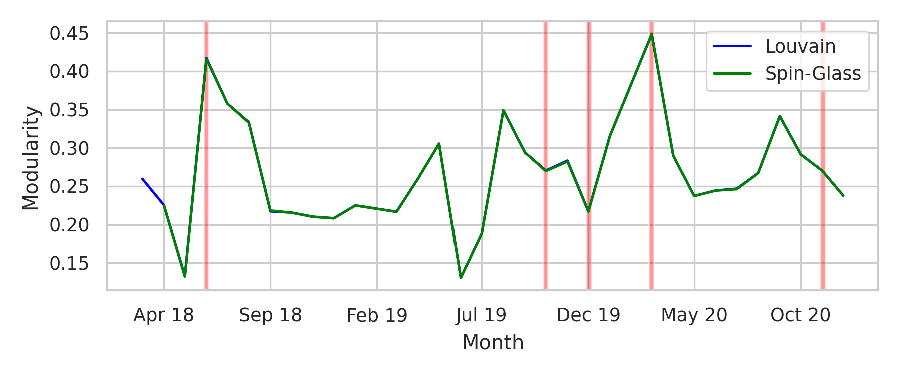
\includegraphics[width=0.95\linewidth]{mod.pdf} 
    \vspace{-5mm}
    \caption{Modularidad obtenida luego de detectar comunidades con cada algortimo, en el tiempo. Las franjas rojas representan meses en que ocurrieron hitos políticos.}
    \label{modfig}
\end{figure}
\begin{figure}[h!]
    \centering
    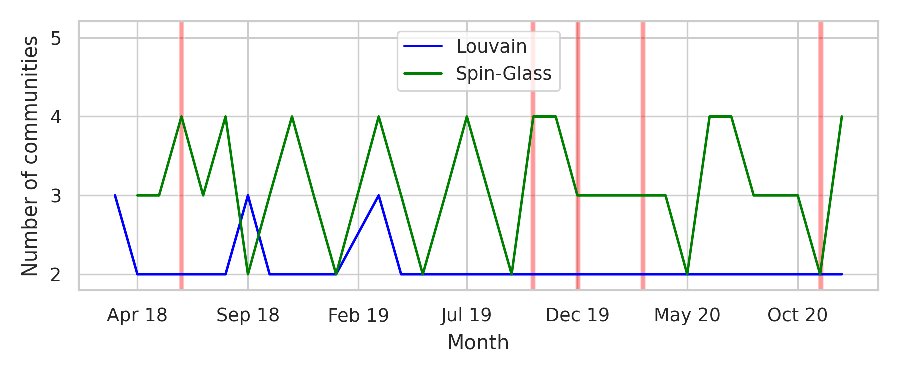
\includegraphics[width=0.95\linewidth]{N.pdf} 
    \vspace{-5mm}
    \caption{Numero de comunidades detectada por cada algorítmo, en el tiempo. Las franjas rojas representan meses en que ocurrieron hitos políticos. Las franjas rojas representan meses en que ocurrieron hitos políticos.}
    \label{N}
\end{figure}

Primero notamos que los 2 métodos son practicamente idénticos para los efectos de calcular la modularidad, habiendo mayores diferencias en en el número de comunidades detectadas. Se pudoinferir que el método Sping-Glass es mucho más sensible para la detección de comunidades, ya que este número fluctua mucho más que para el otro algoritmo. Sin embargo, también se puedo apreciar que los peaks más altos de modularidad (Sep ’18 y Marzo ’20) coinciden con una baja del numero de comunidades respecto a los meses anteriores.

Por otro lado, estos dos meses fueron bastante activos en terminos legislativos. Desde Diciembre de 2020 hasta Marzo de 2020 el parlamento aprueba el cambio el cambio constitucional que prmitiría el nuevo proceso constituyente, y tambien
discute aspectos relevantes de este, como la paridad de genero, siendo esta aprobada en marzo. Durante Junio de 2018, el parlamento intenta responder a las demandas del movimiento feminista que desde Mayo de ese año ya habia generado grandes manifestacion a lo largo de todo Chile. En esta ocasión, un grupo de parlamentarios presenta un proyecto de aborto libre, lo que genero harta controversia mediática.\\

Es importante mencionar que para este análisis no se consideraron todas las votaciónes dentro de cada mes. En concreto, se usaron solo las votaciones con al menos 130 parlamentarios presentes (de un total de 155). También se ignoraron las votaciones cuya opción mayoritaria obtuviese mas del 95\% de lo votos. 

Los resultados fueron muy sensibles a estos dos filtros (cantidad de parlamentarios presentes, porcentaje de la opción mayoritaria). Al variar muy poco estos parámetros, los resultados cambiaron mucho. Algo similar ocurrió al cambiar el intervalo de tiempo que contemplaba cada red (de un mes a un periodo de dos semanas, por ejemplo), probablemente por que no todas las semanas (o meses) hay la misma cantidad de votaciónes en la Cámara. La sensibilidad a estos parámetros es un punto que también se espera estudiar con mayor detalle en este proyecto. 



\subsection{Sugerencia de plan de trabajo}
\begin{itemize}
\item \textbf{Semestre Otoño, 2022.} Este semestre será dedicado para retomar el análisis de redes complejas, a partir del trabajo ya realizado. Se espera crear las redes con la nueva metodología, y poder comparar las medidas de modularidad e índice del triángulo.

\item \textbf{Semestre Primavera, 2022.} En este semestre se estudiará en mayor detalle los distintos algoritmos de detecciónde comunidades, y se espera poder desarrollar el nuevo algoritmo.Se priorizará el desarrolo teórico antes que una implementación computacional.
En este periodo se contempla la redacción de tesis. En caso de ser necesario, esto último pude desarrollarse en parte del siguiente semestre (Otoño 2023). 
\end{itemize}

\subsection{Materiales y financiamiento}

Para llevar a cabo este proyecto se necesitan utilizar las dependencias del Departamento de Física en la Facultad de Ciencias de la Universidad de Chile. % Principalmente, el trabajo se desarrollará en la oficina y los computadores del grupo de investigación PLANETS con acceso a internet.

\subsubsection*{Recursos materiales}

\begin{itemize}
\item Puesto de trabajo y materiales en oficina
%\item Acceso al Cluster en el departamento de Física de la universidad de Chile, para realizar cálculos numéricos y análisis de datos.

%\nocite{*}
\end{itemize}
\subsubsection*{Financiamiento}
\begin{itemize}
\item
\end{itemize}

\bibliographystyle{ieeetr}
\bibliography{refs.bib}
%\printbibliography

\end{document}


 
 
 
 
 
 
